\documentclass{article}
\usepackage[utf8]{inputenc}
\usepackage{graphicx}
\title{A Novel Solution To A Geometric Problem}
\author{Udit Gupta \and Matthew Zhang}
\date{November 2018}

\begin{document}

\maketitle


\section*{Introduction}
The following problem was presented as a challenge to all Centennial students. We chose to write our solution as it was described to be a unique approach.
\begin{center}
	How many ways can one find angle theta?
	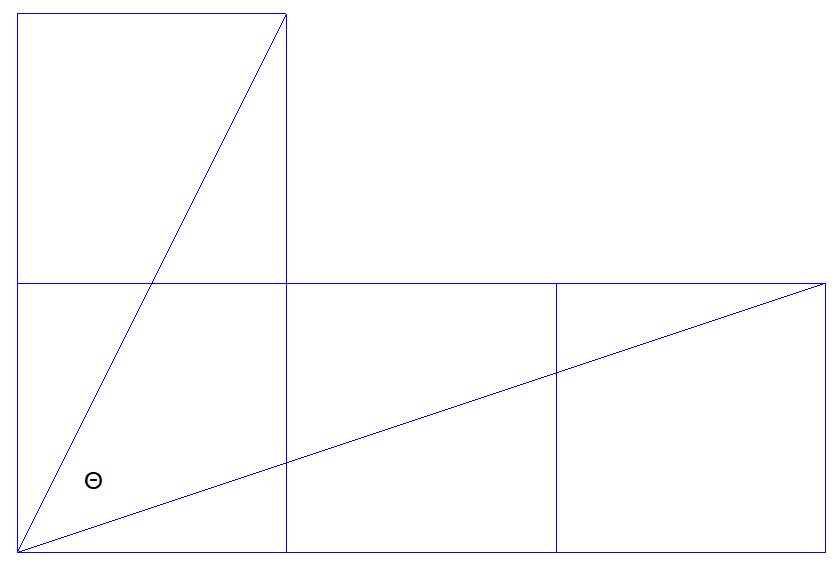
\includegraphics[width=.8\linewidth]{originalTheta.png}
\end{center}

\section*{Solution}
To begin, one must superimpose a Cartesian Plane over the original diagram given alongside the challenge. We will assume the bottom left corner to be the origin in this paper

Now, we can assume the side length of each square to be some constant variable x.

\pagebreak

Utilizing this assumption, one can generate continuous functions that model the line segments. A simple approach of rise over yields the equations below:
 Segment 1: $$ y=2x$$
 Segment 2: $$  y=\frac{1}{3}x$$
\begin{center}
	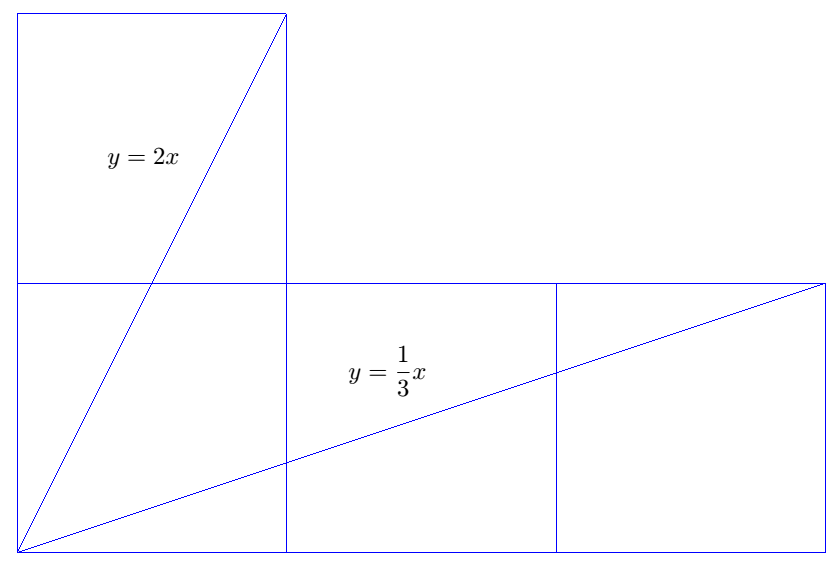
\includegraphics[width=.8\linewidth]{equations.png}
\end{center}

Now, one can impose a circle with radius r $$x^2+y^2=r^2$$
\begin{center}
	\includegraphics[width=.8\linewidth]{circle.png}
\end{center}

\pagebreak
One can create a chord connecting equations 1 and 2. The chord will be referred to as chord a. 
\begin{center}
	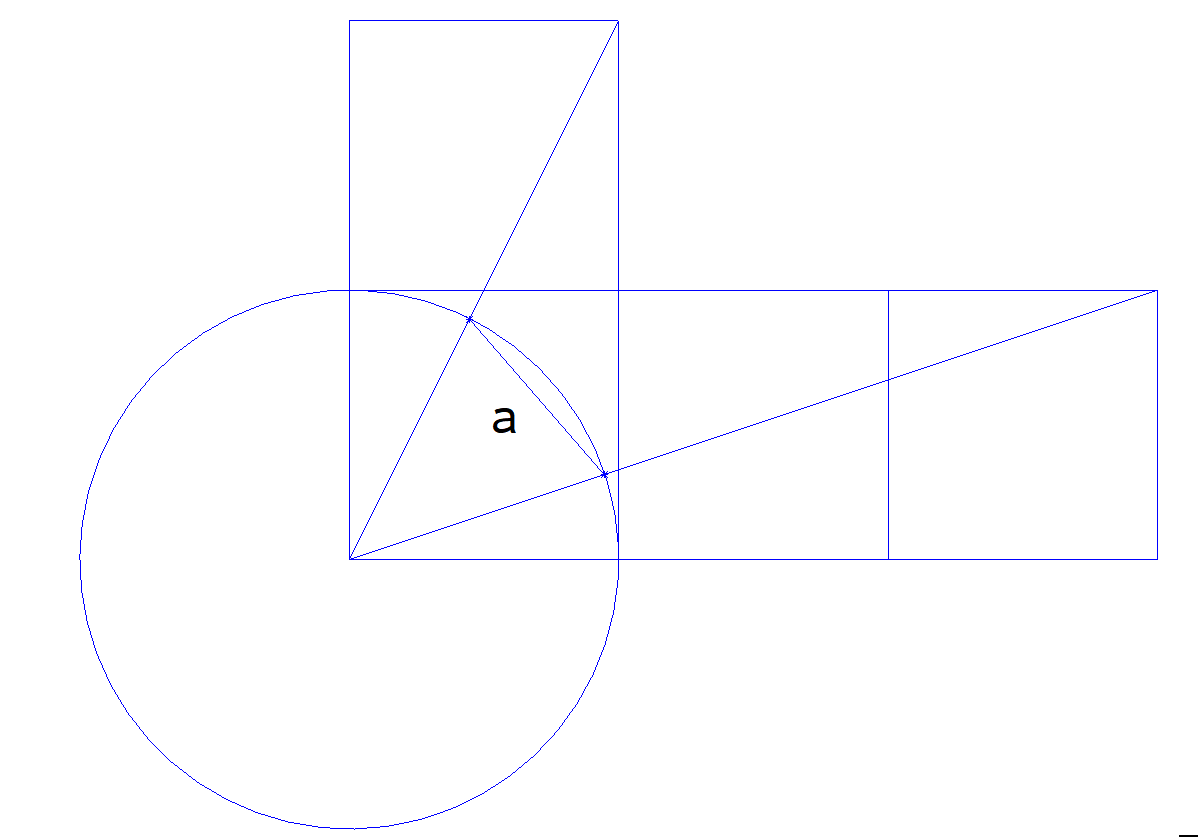
\includegraphics[width=.8\linewidth]{chord.png}
\end{center}

 Utilizing the distance formula, one can find the length of the chord a, but first one must find the points of intersection. 
 
$$ y=2x $$
$$ x^2+y^2=r^2 $$

This yields one point $$(\frac{ r\sqrt{5} }{5}, \frac{ 2r\sqrt{5} }{5})$$

For the other line we have
$$ y=(1/3)x $$
$$ x^2+y^2=r^2 $$



This yields the point: $$(\frac{3r\sqrt{10}}{10}, \frac{r\sqrt{10}}{10})$$

Now, one can use the distance formula:

$$ a=\sqrt{(\frac{ r\sqrt{5} }{5}-\frac{3r\sqrt{10}}{10})^2 + (\frac{ 2r\sqrt{5} }{5}-\frac{r\sqrt{10}}{10})^2}$$


To avoid confusion, we will not simplify this solution. Instead, we will now move on to the next step which requires the Law of Cosines.

$$ a^2=b^2+c^2-2bccos\theta$$

\pagebreak

a is the length of the cord while b and c are the radius,r, of the circle. Solving and simplifying this equation leaves us with the solution:
 \begin{center}

\includegraphics[width=.8\linewidth]{solution.png}
 \end{center}

$$\theta=45^o$$
\end{document}
